% ICMC 2004 paper template for Latex2e.

% Points to note:
%    Please use \paragraph instead of \subsubsection -- see discussion below.
%    See comments in the References section on how to do citations.

\documentclass[10pt,letterpaper]{article}
\usepackage{fullpage}
\usepackage{times}
\usepackage{chicago}                    % for "(Author, year)" cite style.
\usepackage{indentfirst}                % indent para after headings.
% alex put this here
\usepackage{graphicx}
\setlength{\textheight}{10in}
% \usepackage{url}                      % (handy if you reference a URL.)

\setlength{\oddsidemargin}{-0.25in}     % Latex has one-inch "driver margin"
% \setlength{\evensidemargin}{-0.25in}  % (shouldn't be necessary)
\setlength{\textwidth}{7in}             % 8.5 - 2*0.75 

\setlength{\columnsep}{0.25in}
\setlength{\parindent}{0.2in}

\raggedbottom                           % better than inter-para spaces, I say.


\begin{document}

\twocolumn

\title{\textbf{ATS user interfaces}}
\author{
Pete Moss and Alex Norman\\
DxArts, University of Washington\\
pete@petemoss.org\\
School of Computer Science and Engineering, University of Washington\\
alexnorman@users.sourceforge.net\\
}
\date{}     % no date
\maketitle

\pagestyle{empty}          % no page numbers.
\thispagestyle{empty}      % yes, that includes not on the first page, either.


\section{ats-csound}
Alex Norman has written several csound unit generators that extract data from ATS files.  Many of these u-gens are derived from, and work much like Richard Karpen's phase vocoder unit generators for csound (pvread, pvadd etc.).  As with pvread etc., most of the ats-csound u-gens take a "time pointer" that is used to index data from ATS data files.  Linear interpolation is used to approximate data between analysis frames.

The csound unit generators can be broken down into two groups: those that act independently, and those that depend on the unit generator atsbufread.

\subsection{Independent Unit Generators}
All of the independent u-gens take an ATS file and a time pointer as arguments.  Using these and other arguments, the u-gens extract data from an ATS file at the time indicated by the time pointer.

\textbf{atsread} and \textbf{atsreadnz} are the most generic u-gens in the ats-csound package.  Each of these u-gens simply read data (with interpolation) out of an ATS data file and return it for arbitrary use.  atsread returns the frequency and amplitude information of a user specified partial.  atsreadnz takes a noise band number and returns the corresponding noise energy data.

\textbf{atsadd} and \textbf{atsaddnz} use data from ATS analysis files to synthesize sine-waves or noise respectively.  atsadd uses a standard interpolated table look up synthesis method to synthesize an array of sinusoids that are combined additively to produce a single audio rate output.  The user specifies a range of partials to synthesize.  The frequency and amplitude information for these partials are taken from a given ATS data file.  A frequency multiplier, given by the user, is used before synthesis to transpose the data in frequency.

Like pvadd, atsadd provides an optional amplitude "gate" function.  This "gate" function is given by a csound f-table and is used to scale the partials' amplitudes.  Amplitudes are normalized based on the maxim amplitude in the analysis file.  The gate function uses these normalized amplitudes to index the provided f-table.  A partial with an amplitude of 0 will index first data point in the f-table, a partial with the maximum amplitude in the analysis file will index the last position in the f-table.  The value of the indexed data is used to scale the amplitudes before synthesis.  With this "gate" function a user can distort the re-synthesis in subtle or extreme ways.

atsaddnz synthesizes a set of noise bands indicated by the user.  It does this using an array of band limited noise bands that are modulated by sine waves to be put into the correct place in the frequency spectrum.  These bands are combined additively to produce a single audio rate output.  The range of bands in the synthesis is determined by the user.

\textbf{atssinnoi} synthesizes sine waves and noise together in a unique manner.  First the partials are sorted into groups depending on which frequency band they are in.  Second, the noise energy from each band is distributed equally among each of the partials in that band.  Third, each partial is synthesized using an internal oscillator.  Fourth, for each partial a noise band is synthesized who's bandwidth is determined by a function of the partial's frequency and energy is determined by the method described earlier.  Fifth, the noise bands are modulated by their corresponding partial's sine-wave.  Finally, after being scaled appropriately, all of the sine-waves and noise bands are added together to give a single audio rate output.

Just as with atsadd a frequency multiplier can be used to transpose the data in frequency.  Also, using provided k-rate inputs, a user can scale the total amplitude of the sine-waves and noise independently of each other after the noise modulation occurs.

The final independent unit generator \textbf{atsbufread} has no outputs that are directly accessible by the user.  atsbufread takes data from an ATS file and produces a table of partials' amplitude and frequency values in memory.  This memory can be accessed by other unit generators.  Like atsadd, atsbufread uses a time pointer and a users specified list of partials to produce the table.  The next section will describe the unit generators that operate on data provided by atsbufread.

\subsection{atsbufread Dependent Unit Generators}
\textbf{atsinterpread} takes a single argument, a frequency value.  Using this frequency value atsinterpread indexes a table produced by an atsbufread u-gen and returns the corresponding amplitude value.  Interpolation is used for in between values.  This u-gen can be useful for cross synthesizing non ATS derived signals with data from ATS.

\textbf{atspartialtap} works almost exactly like atsread except it reads it's data from a table produced by an atsbufread.  The only argument this u-gen takes is a partial number; it returns frequency and amplitude data.  This u-gen is useful if a user wants to operate on multiple partials separately but have them use the same time pointer.  While this can easily be achieved with an array of atsreads all using the same time pointer, its simplicity makes it attractive.

\textbf{atscross}, based on pvcross, allows a user to perform cross synthesis using the data from two ATS files.  One of these ATS files comes from the atsbufread, the other is provided by the atscross unit generator.  Data is extracted from the ATS file indicated by the atscross u-gen, and used to index the table produced by the atsbufread u-gen in the same way as atsinterpread indexes the table.  Now each partial from the ATS file provided by the atscross u-gen has two amplitudes, the original amplitude from its data file and the amplitude interpolated from the ATS file of the corresponding atsbufread u-gen.  Each of these amplitudes is then scaled independently by user specified k-rate values.  The amplitudes are then summed and used, with the frequency of the corresponding partial, for synthesis.  Synthesis is then achieved using the same method as atsadd.  In fact, if the user gives a scalar value of 1 for the atscross ATS file's amplitude and a 0 scalar value for the atsbufread ATS file's amplitude this u-gen acts exactly like atsadd.  But if a value of 0 is given for the scalar value for the atscross ATS file's amplitude and a value of 1 is given for the atsbufread ATS file's amplitude, all the frequency data will come from the atscross file but all the amplitude data will come from the atsbufread.  Scalar values can be varied to achieve morphing from a standard atsadd sound to a cross-synthesized sound.

\section{ats-pd}
Alex Norman has created an object for Pure-Data that allows users to access data in a similar way to the csound u-gens atsread and atsreadnz.  This pd object is called \textbf{atsread}.

\textbf{atsread} uses a time pointer exactly the same way that its csound counter part does.  The pd version combines the functionality of the csound atsread and atsread noise.  In addition to it's combined functionality the pd object can output lists of data, allowing for one object to output all the partial and noise data for one file.  atsread for pd has three outputs: the first output gives a list of frequency values, the second gives a list of corresponding amplitude values, and the third gives a list of noise energy values.  The lists are always given in order from lowest partial/band to highest partial/band.  The user opens an ATS file for access by sending a message in this format: "open cl.ats", alternatively the ATS file name can be given as an argument to the object.  A user can set a range of partials by giving messages of the form "set 1 2 5 10..20".  This example would output partials 1, 2, 5, and 10-20 (if they exist in the data file).  Partials can be added to be output using messages of the form "add 3 4..7 9".  This would add partials 3, 4-7 and 9 to be output, and continue outputting the partials that were being output before.  Finally partials can be removed from the output by using messages of the form "remove 4..6 11 13".  The same operations can be performed on noise bands by appending an "nz" to the first argument of the message, IE. "setnz 1 2 17".

The pd atsread object can also be made to only output noise or sine-waves using the "nosines", "nonoise", "sines" and "noise" messages.  "nosines" turns off frequency and amplitude outputs, "sines" turns them back on.  Similarly "nonoise" turns off noise outputs, "noise" turns them back on.  These messages can also be given as arguments to the object.

Just as with the csound atsread function the user is left to do what he/she wants with the data.  Synthesis easily be preformed with a bank of oscillators, though the data could also be used as control data for other operations.


\begin{figure}[htb]
	\begin{center}
	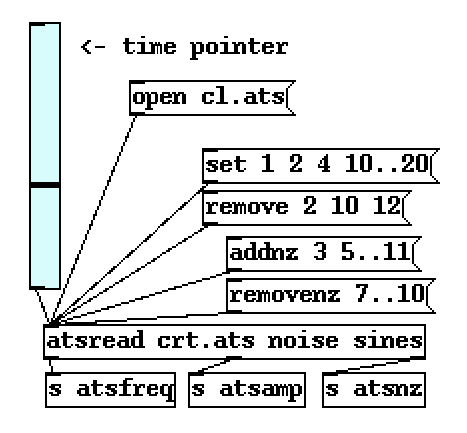
\includegraphics{ats-pd-example.eps}
	\caption{atsread pd interface example.}
	\label{fig:emptybox}
	\end{center}
\end{figure}

\end{document}
